\chapter{System Design}

\section{Design Goals}
The design of DeepSceneLoc emphasizes modularity, reproducibility, and phased extensibility. Stage 1 is intentionally engineered as a stable semantic engine that can be reused by Stage 2 exact-location reasoning.

\section{High Level Architecture}
The pipeline is divided into independent modules:
\begin{itemize}
\item Data preparation and class mapping.
\item Preprocessing and augmentation.
\item Model training and checkpointing.
\item Evaluation and visualization.
\item Demo inference interface.
\end{itemize}

This modular separation reduces coupling and enables targeted upgrades without breaking end to end execution.

\section{Component Level Architecture}
At implementation level, the system can be represented as five cooperating components:
\begin{itemize}
\item \textbf{Ingestion component:} handles input validation and class-folder organization.
\item \textbf{Transformation component:} applies deterministic preprocessing and stochastic augmentation.
\item \textbf{Modeling component:} encapsulates architecture construction, forward pass, and checkpoint restoration.
\item \textbf{Evaluation component:} computes metrics, confusion matrices, and serializable reports.
\item \textbf{Presentation component:} renders human-readable outputs for demonstration.
\end{itemize}

Each component has explicit interfaces to prevent hidden coupling. This design improves maintainability and supports unit-level debugging when behavior changes after hyperparameter or model updates.

\section{Data Flow Design}
The report includes DFD content at three abstraction levels derived from the latest project diagram specifications.

\subsection{Design Diagram Summary}
The design diagrams are included directly in this report as local assets so they remain stable when the report is shared.

\subsection{DFD Level 0: Context}
At the context level, DeepSceneLoc interacts with four external entities: user/developer, Places365 dataset, GitHub repository, and Gemini API (planned in Stage 2). The user provides an image to the system, and the system returns scene/location output.

\subsection{DFD Level 1: Main Processes}
The main pipeline is decomposed into seven major processes:
\begin{itemize}
\item Process 1: dataset preparation,
\item Process 2: image preprocessing,
\item Process 3: Stage 1 scene classification,
\item Process 4: Stage 2 exact-location reasoning (planned),
\item Process 5: model training,
\item Process 6: result display,
\item Process 7: evaluation and metrics reporting.
\end{itemize}

\begin{figure}[htbp]
\centering
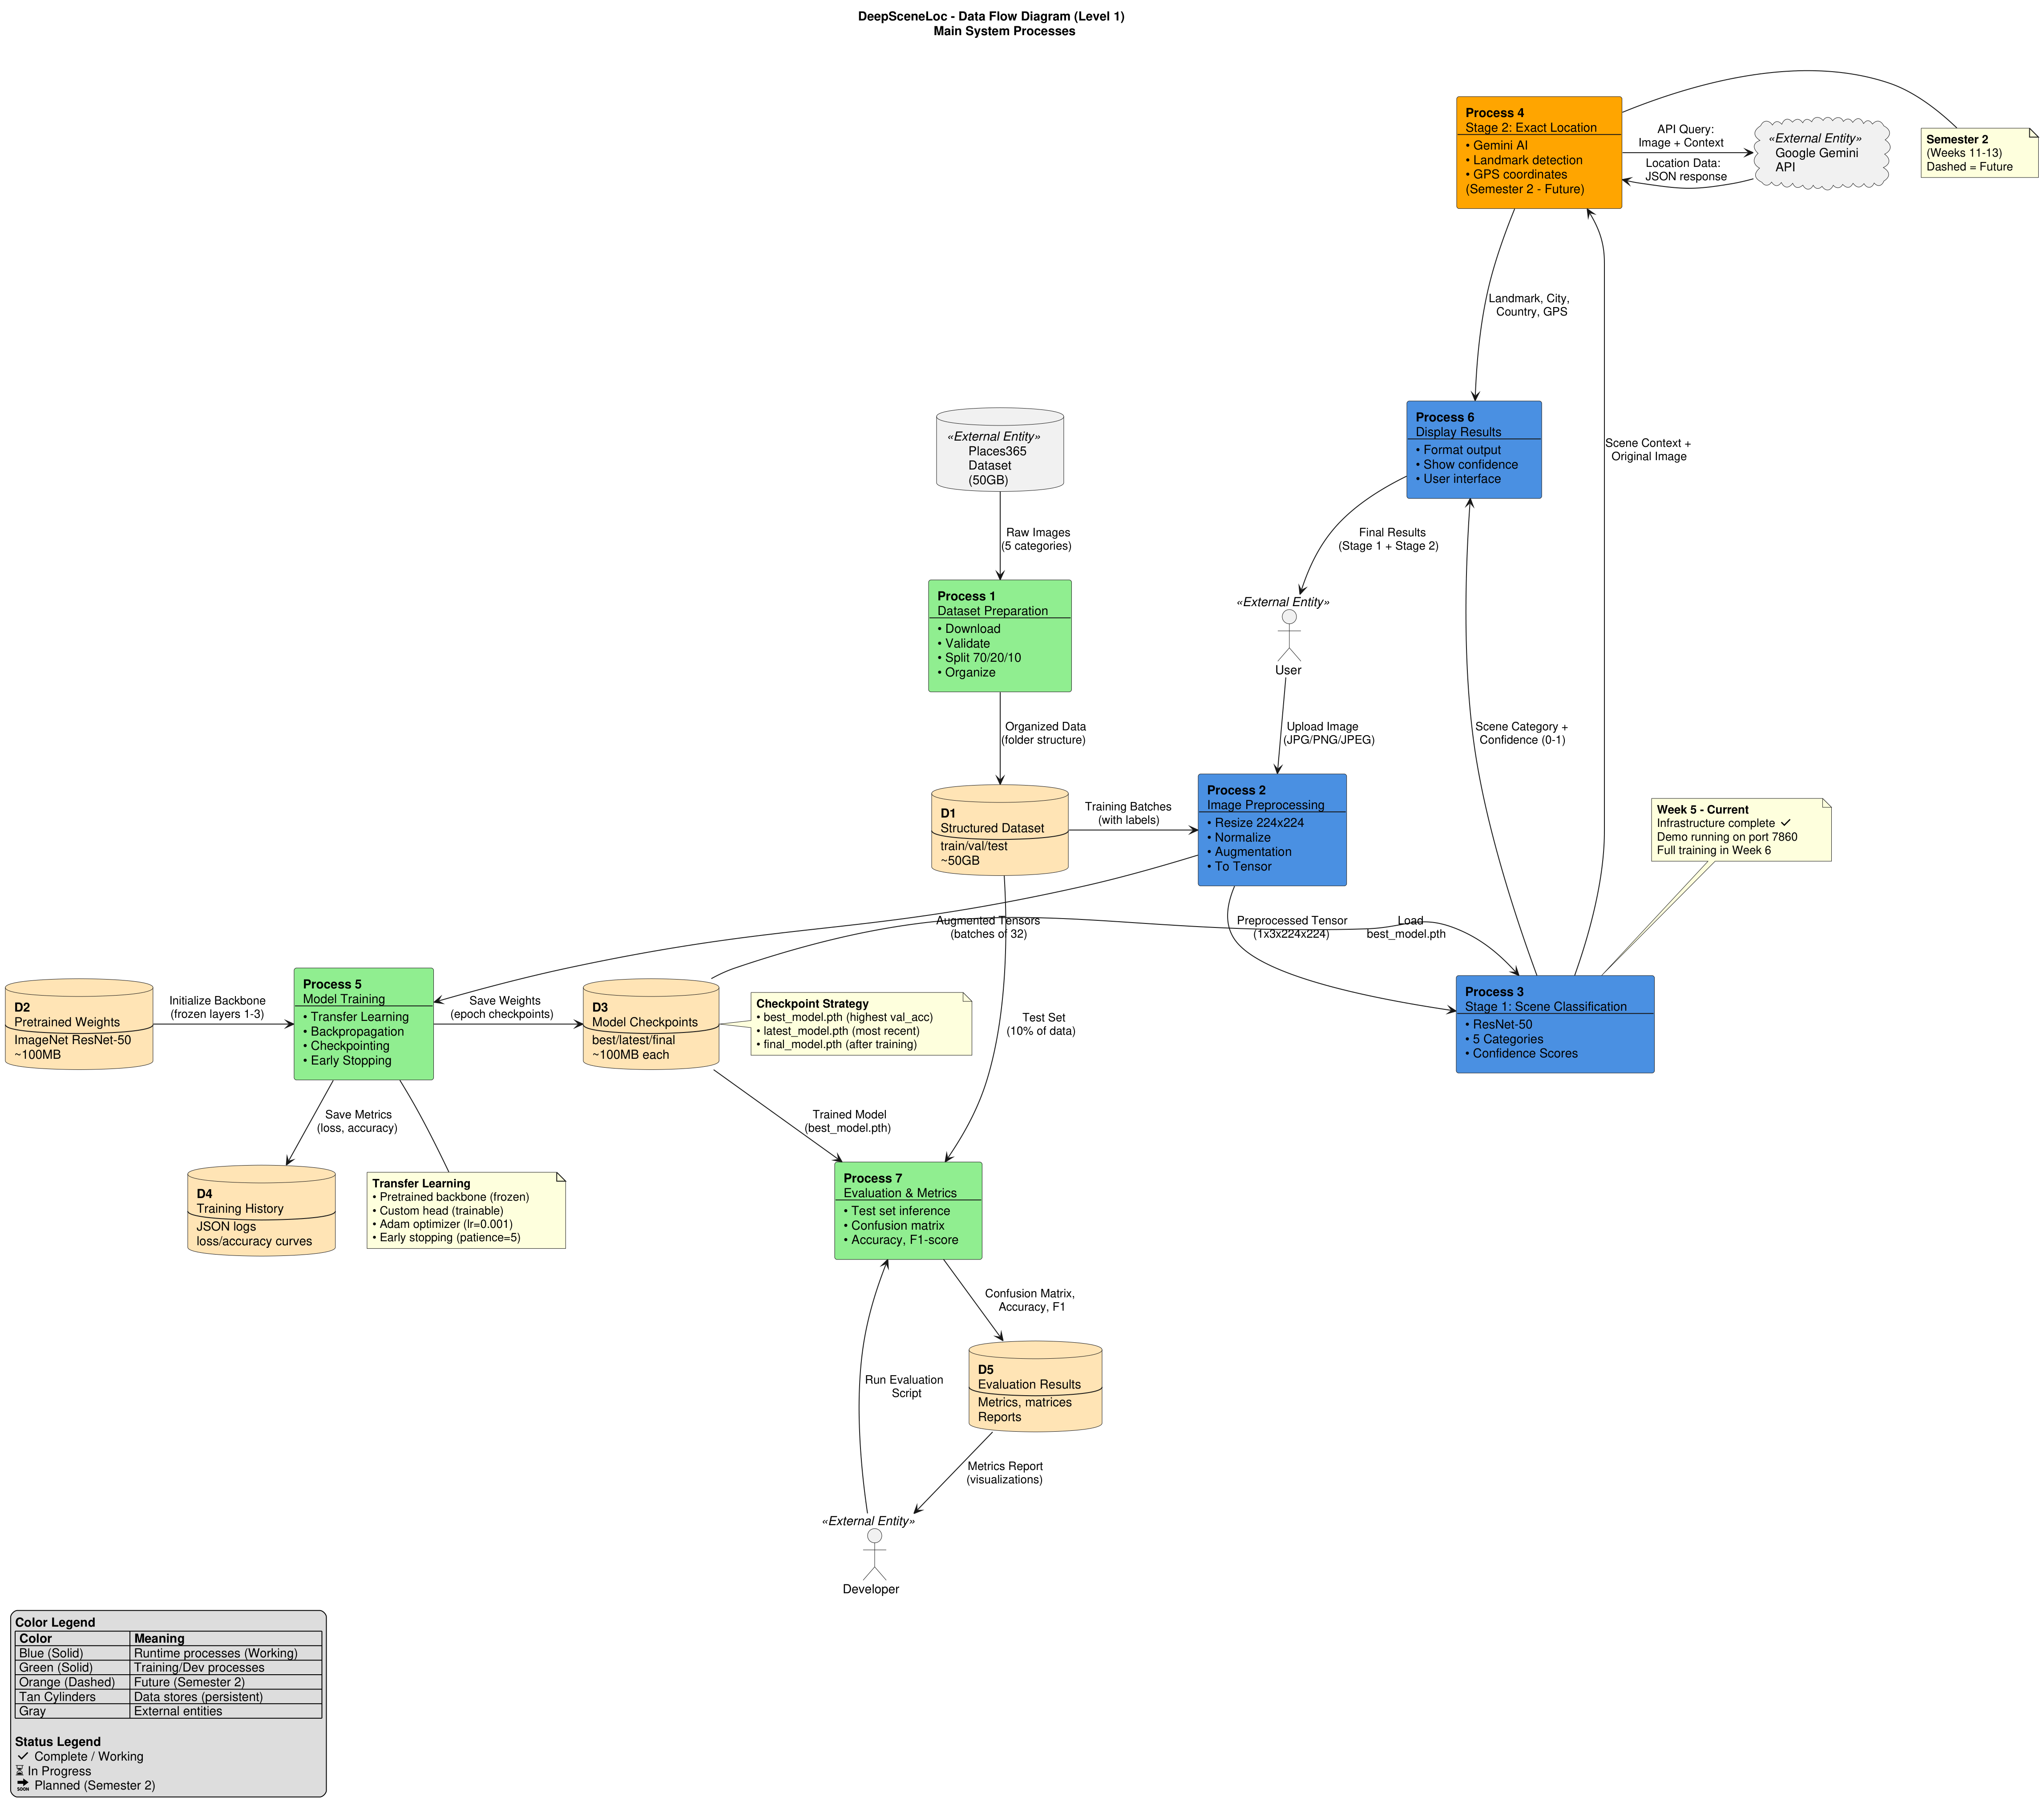
\includegraphics[width=\textwidth]{diagrams/dfd.png}
\caption{DFD Level 1: Main system processes}
\label{fig:dfd-level-1}
\end{figure}
\FloatBarrier

Persistent stores include structured dataset partitions, pretrained weights, model checkpoints, training logs, and evaluation outputs.

\subsection{DFD Level 2: Stage 1 Classification Decomposition}
Stage 1 is further decomposed into validation and inference sub-steps: input tensor validation, model-loading, checkpoint-loading, forward pass, softmax conversion, top-$k$ extraction, confidence validation, and output formatting. Decision nodes handle invalid shape, missing checkpoint, and low-confidence output branches.

\section{Data Contract Design}
The project uses explicit data contracts between modules:
\begin{itemize}
\item input image contract (format, channel count, minimum dimensions),
\item tensor contract (shape and normalization assumptions),
\item output contract (predicted label, confidence vector, top-$k$ ordering),
\item evaluation contract (macro metrics, per-class metrics, confusion matrix).
\end{itemize}

By defining these contracts, the system avoids implicit assumptions that commonly cause integration failure when modules evolve independently.

\subsection{Input Layer}
Raw images are organized into category folders. A mapping file aligns source categories to the five target classes.

\subsection{Preprocessing Layer}
Each image is resized to 224\,$\times$\,224 and normalized using ImageNet statistics. Augmentations are applied during training to improve generalization.

\subsection{Learning Layer}
The ResNet-50 backbone extracts feature representations. A task specific classification head produces class logits, followed by softmax for probability estimation.

\subsection{Output Layer}
The output consists of predicted class, confidence distribution, and artifacts used for model interpretation (confusion matrix and class wise scores).

\section{Model Design}
\subsection{Backbone Selection}
ResNet-50 was selected due to proven transfer-learning behavior, manageable compute requirements, and reliable convergence in medium-scale experiments.

\subsection{Fine-Tuning Strategy}
Lower convolution blocks retain pretrained weights, while deeper layers and the final head adapt to project-specific categories. This strategy accelerates training and reduces overfitting risk.

\subsection{Why This Design Was Chosen}
The baseline design intentionally favors robustness over novelty. A stable ResNet-50 transfer learning pipeline provides a reliable benchmark for the minor phase and leaves sufficient room to evaluate advanced alternatives without changing dataset semantics or reporting criteria. This approach reduces confounding factors and makes comparative analysis more scientifically defensible.

\section{Evaluation Design}
Evaluation includes macro metrics and class-level diagnostics. The design ensures the model is not judged solely by aggregate accuracy but also by balanced class behavior.

\begin{figure}[htbp]
\centering
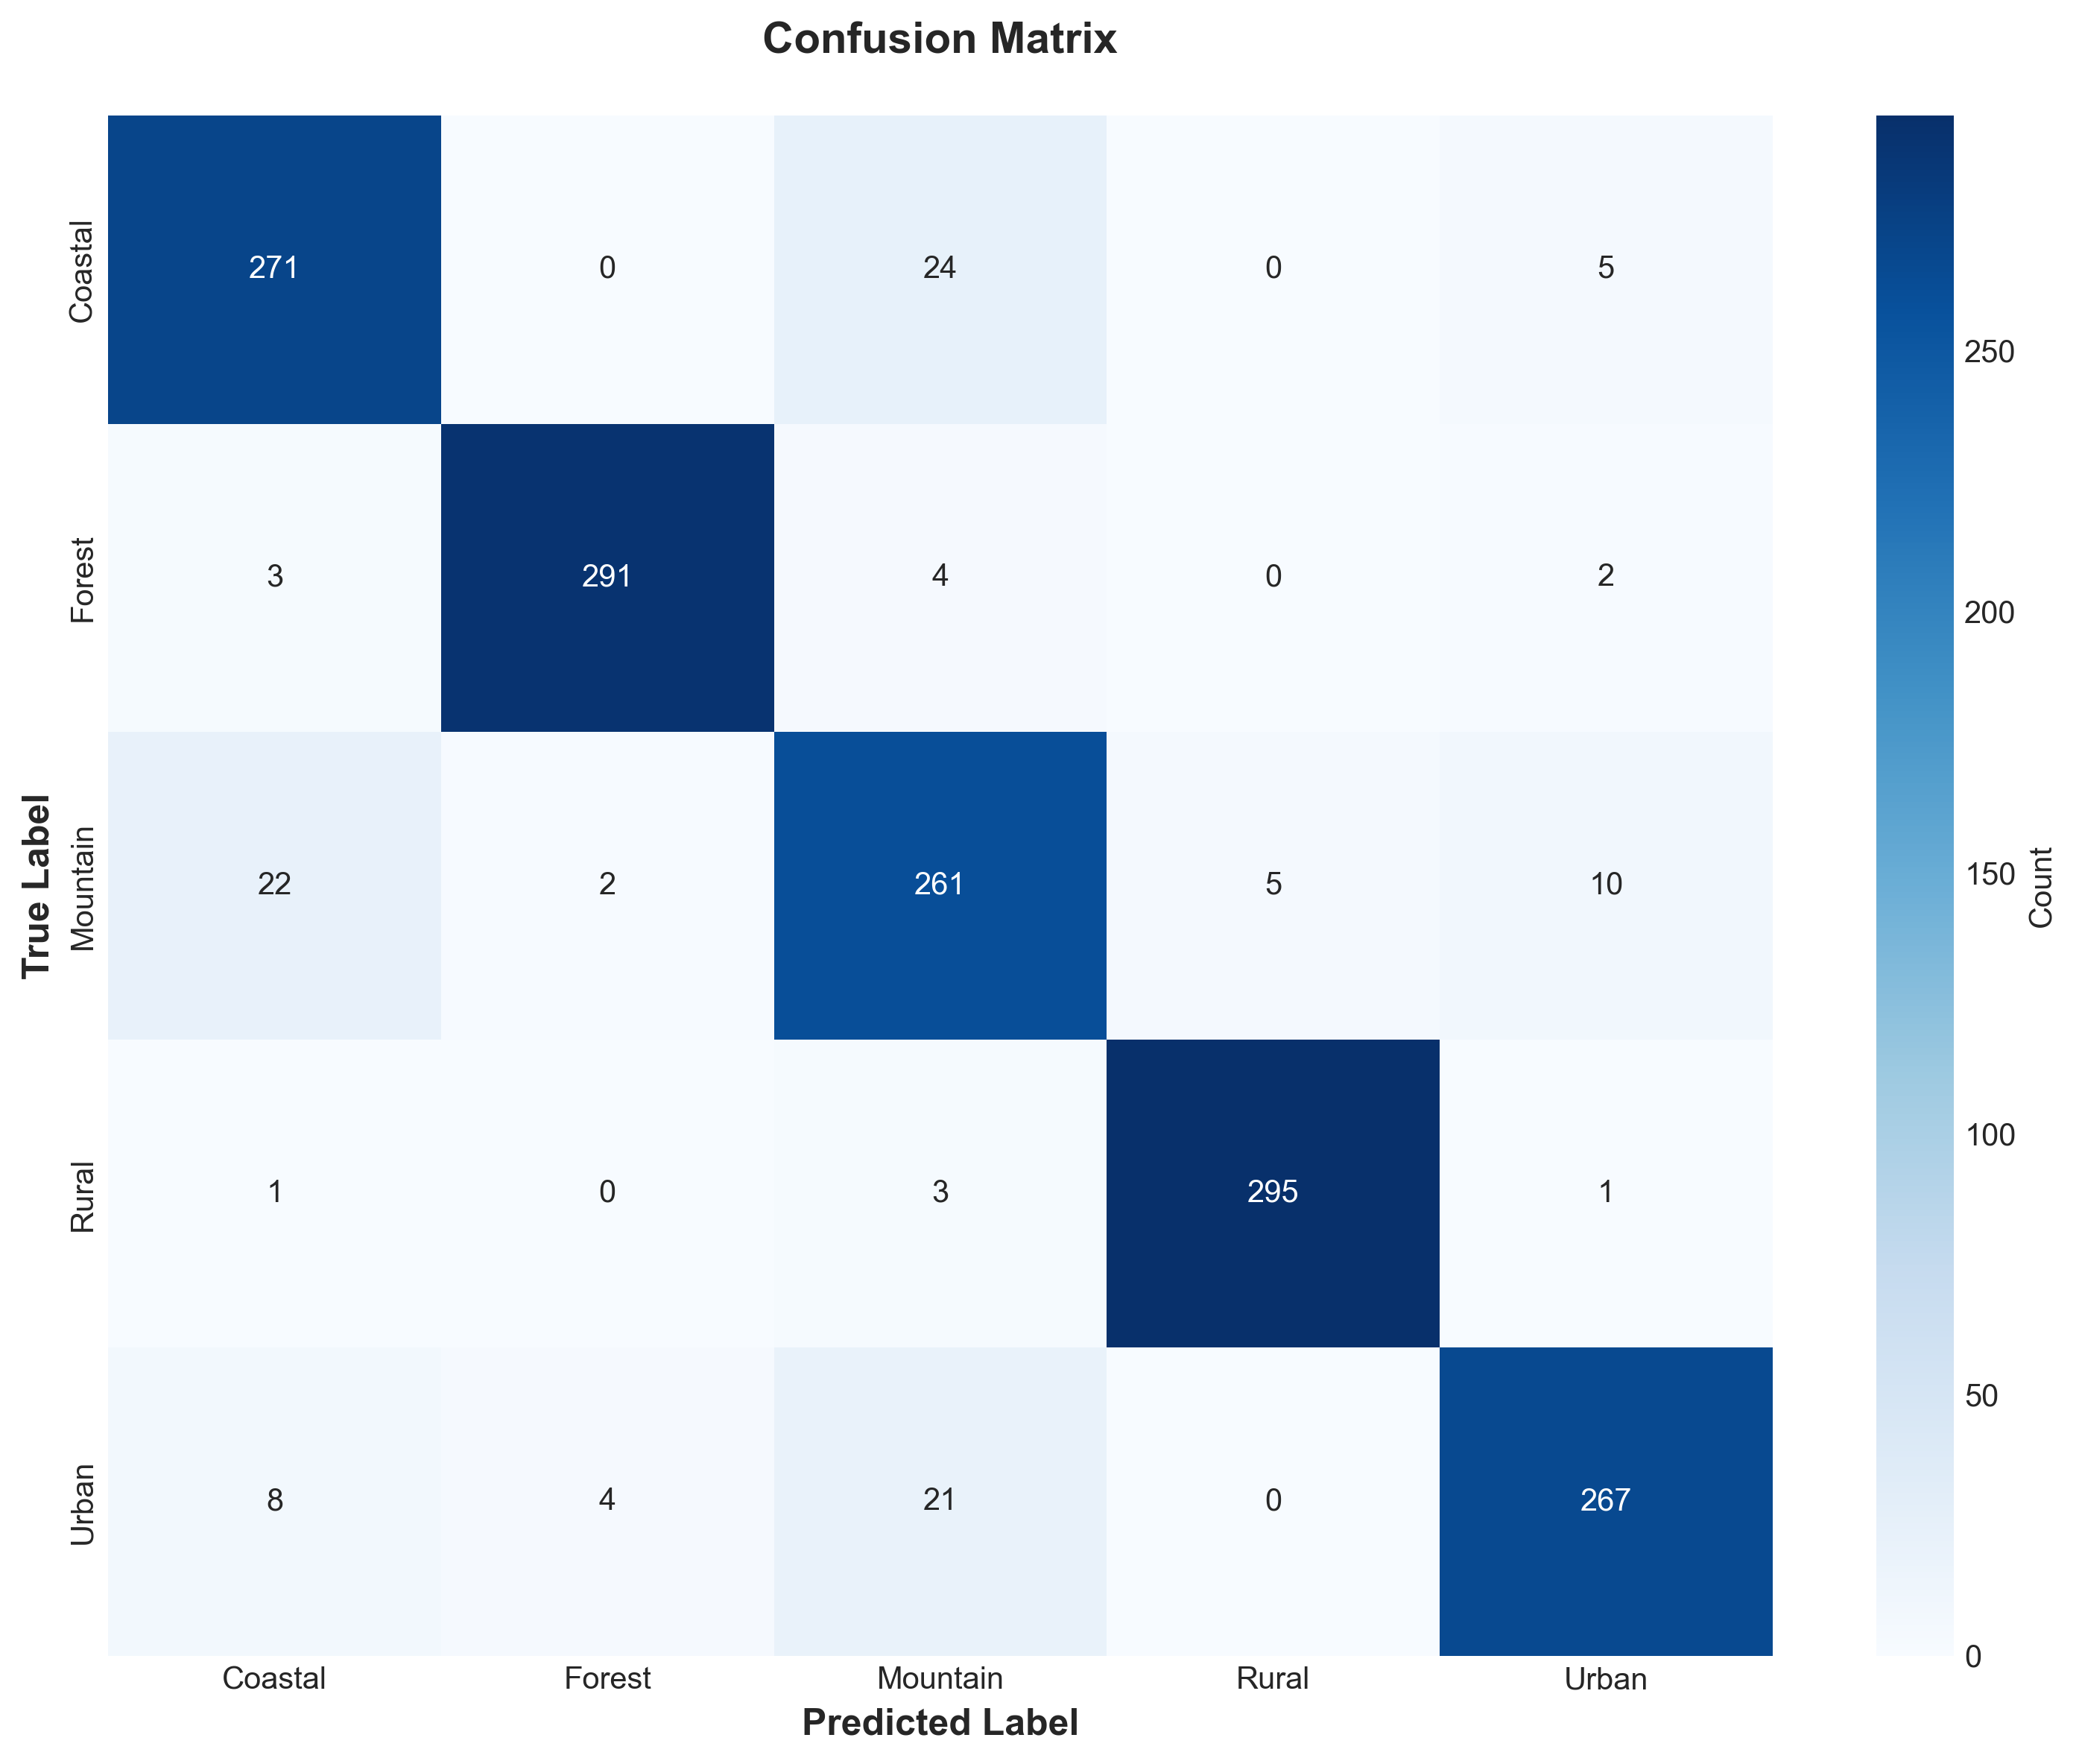
\includegraphics[width=0.78\textwidth]{assets/figures/confusion_matrix.png}
\caption{Confusion matrix for five-class scene classification}
\label{fig:cm-design}
\end{figure}

\begin{figure}[htbp]
\centering
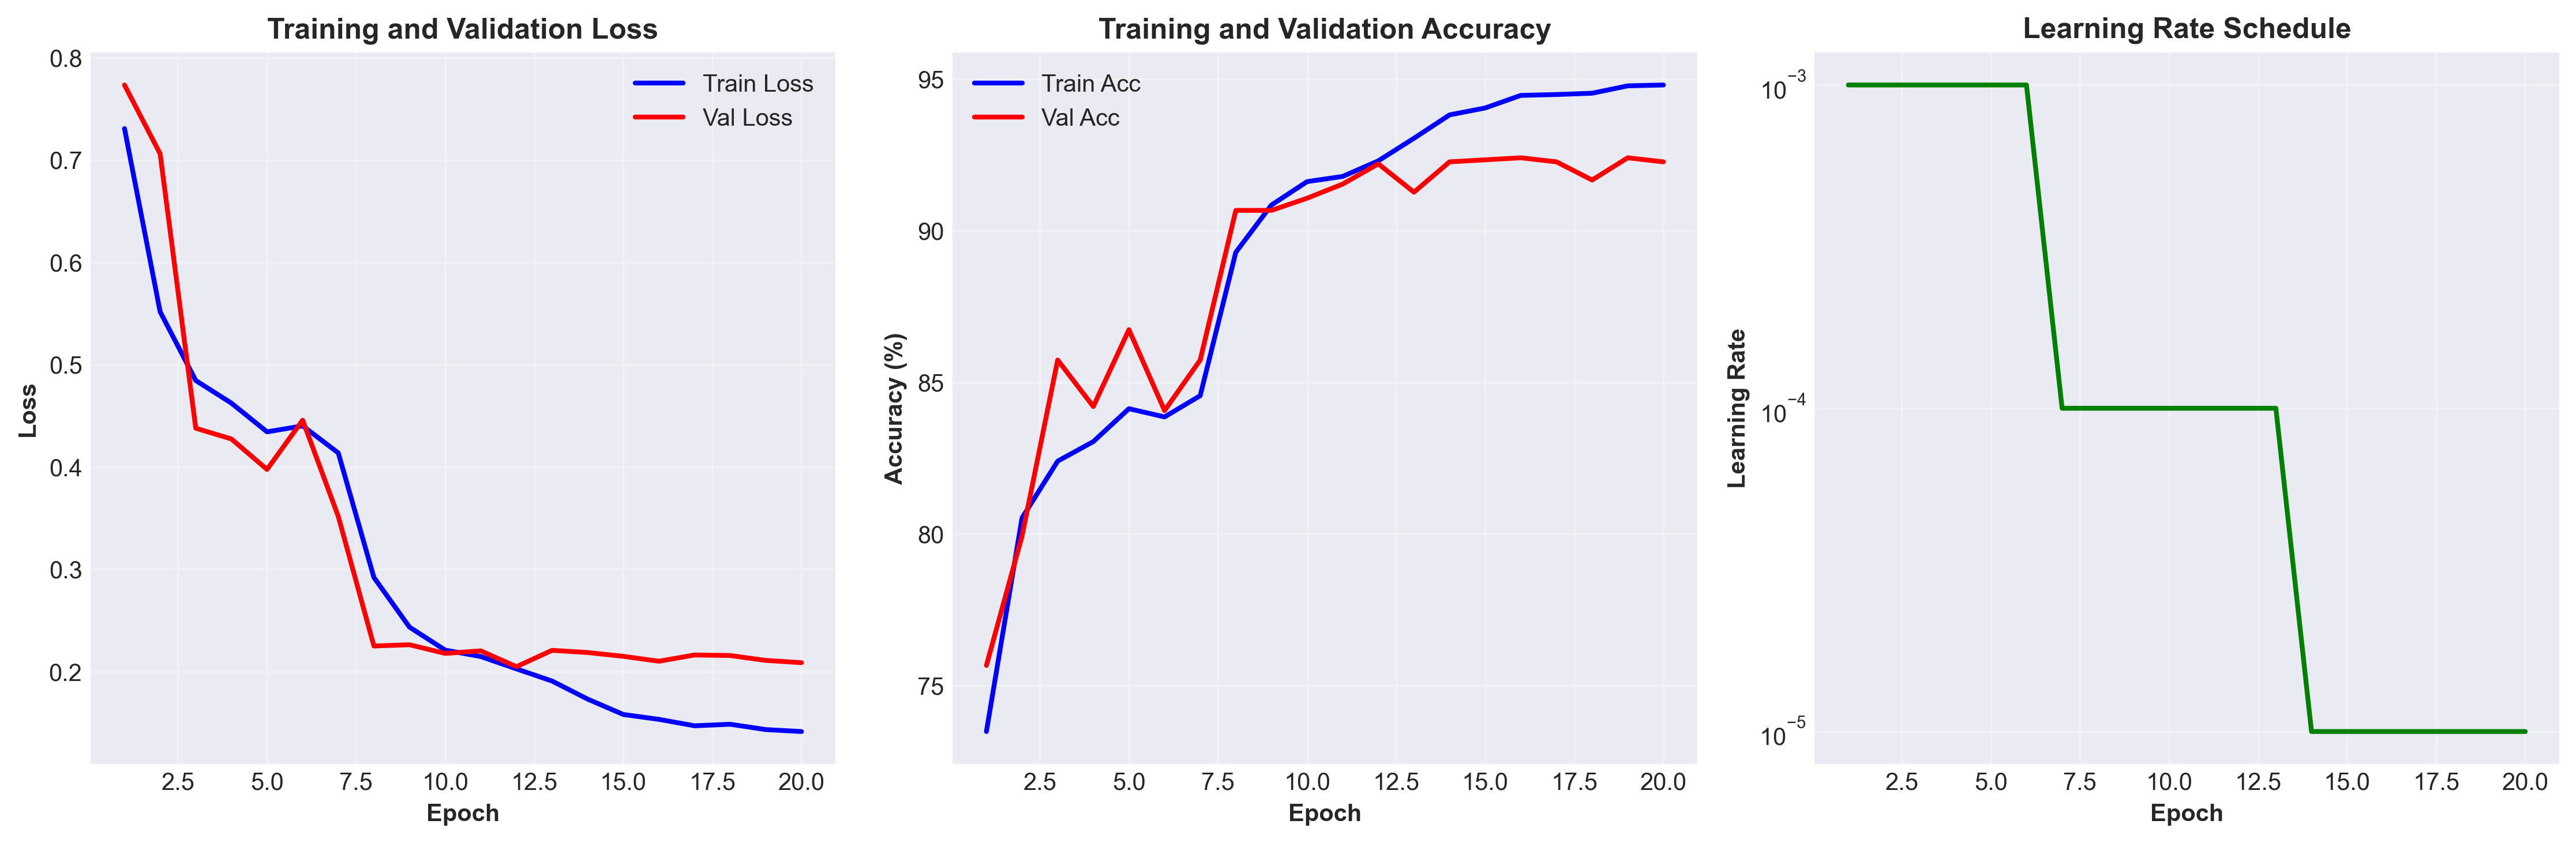
\includegraphics[width=0.78\textwidth]{assets/figures/training_history.png}
\caption{Training and validation curves used for convergence analysis}
\label{fig:history-design}
\end{figure}
\FloatBarrier

\section{Design for Stage 2 Extension}
The current design exports scene class probabilities, which are planned to be consumed by an exact location reasoning module in Semester 2. This allows the future system to condition fine grained geolocation on reliable scene priors.

Stage 2 compatibility also depends on explanation readiness. Therefore, the design preserves confidence distributions and class ranking rather than only top-1 labels. This richer output enables downstream reasoning modules to make safer decisions under uncertainty and to trigger fallback behavior when priors are diffuse.

\section{Chapter Summary}
The design establishes a clean and expandable architecture with measurable interfaces between modules, supporting both current deliverables and next-phase integration.
